\documentclass{beamer}

\usetheme{Boadilla}

\usepackage{times}
\usefonttheme{structurebold}
\usepackage{listings}
\usepackage{listings-rust}

\usepackage{pgf}
\usepackage{tikz}
\usepackage{alltt}
\usepackage[normalem]{ulem}
\usetikzlibrary{arrows,automata,shapes,positioning}
\usepackage{amsmath,amssymb}
\usepackage{rotating}
\usepackage{ulem}
\usepackage{pythonhighlight}
\usepackage{amssymb}
\usepackage{pifont}
\newcommand{\xmark}{\ding{55}}
\usepackage{dafny}

\usetikzlibrary{arrows,automata,shapes}
\tikzstyle{block} = [rectangle, draw, fill=blue!20, 
    text width=5em, text centered, rounded corners, minimum height=2em]
\tikzstyle{bt} = [rectangle, draw, fill=blue!20, 
    text width=4em, text centered, rounded corners, minimum height=2em]

\lstset{ %
language=Rust}

%\setbeamercovered{dynamic}
\setbeamertemplate{footline}[page number]{}
\setbeamertemplate{navigation symbols}{}
\usefonttheme{structurebold}

\title{Software Testing, Quality Assurance \& Maintenance---Lecture 17}
\author{Patrick Lam\\University of Waterloo}
\date{March 9, 2026}

\colorlet{redshaded}{red!25!bg}
\colorlet{shaded}{black!25!bg}
\colorlet{shadedshaded}{black!10!bg}
\colorlet{blackshaded}{black!40!bg}

\colorlet{darkred}{red!80!black}
\colorlet{darkblue}{blue!80!black}
\colorlet{darkgreen}{green!80!black}

\newcommand{\rot}[1]{\rotatebox{90}{\mbox{#1}}}
\newcommand{\gray}[1]{\mbox{#1}}

\newenvironment{changemargin}[1]{% 
  \begin{list}{}{% 
    \setlength{\topsep}{0pt}% 
    \setlength{\leftmargin}{#1}% 
    \setlength{\rightmargin}{1em}
    \setlength{\listparindent}{\parindent}% 
    \setlength{\itemindent}{\parindent}% 
    \setlength{\parsep}{\parskip}% 
  }% 
  \item[]}{\end{list}}

\newcommand{\brac}[1]{\texttt{\textless #1\textgreater}}


\begin{document}
\begin{frame}
  \titlepage
\end{frame}

%\usebackgroundtemplate{\tikz\node[opacity=0.3]{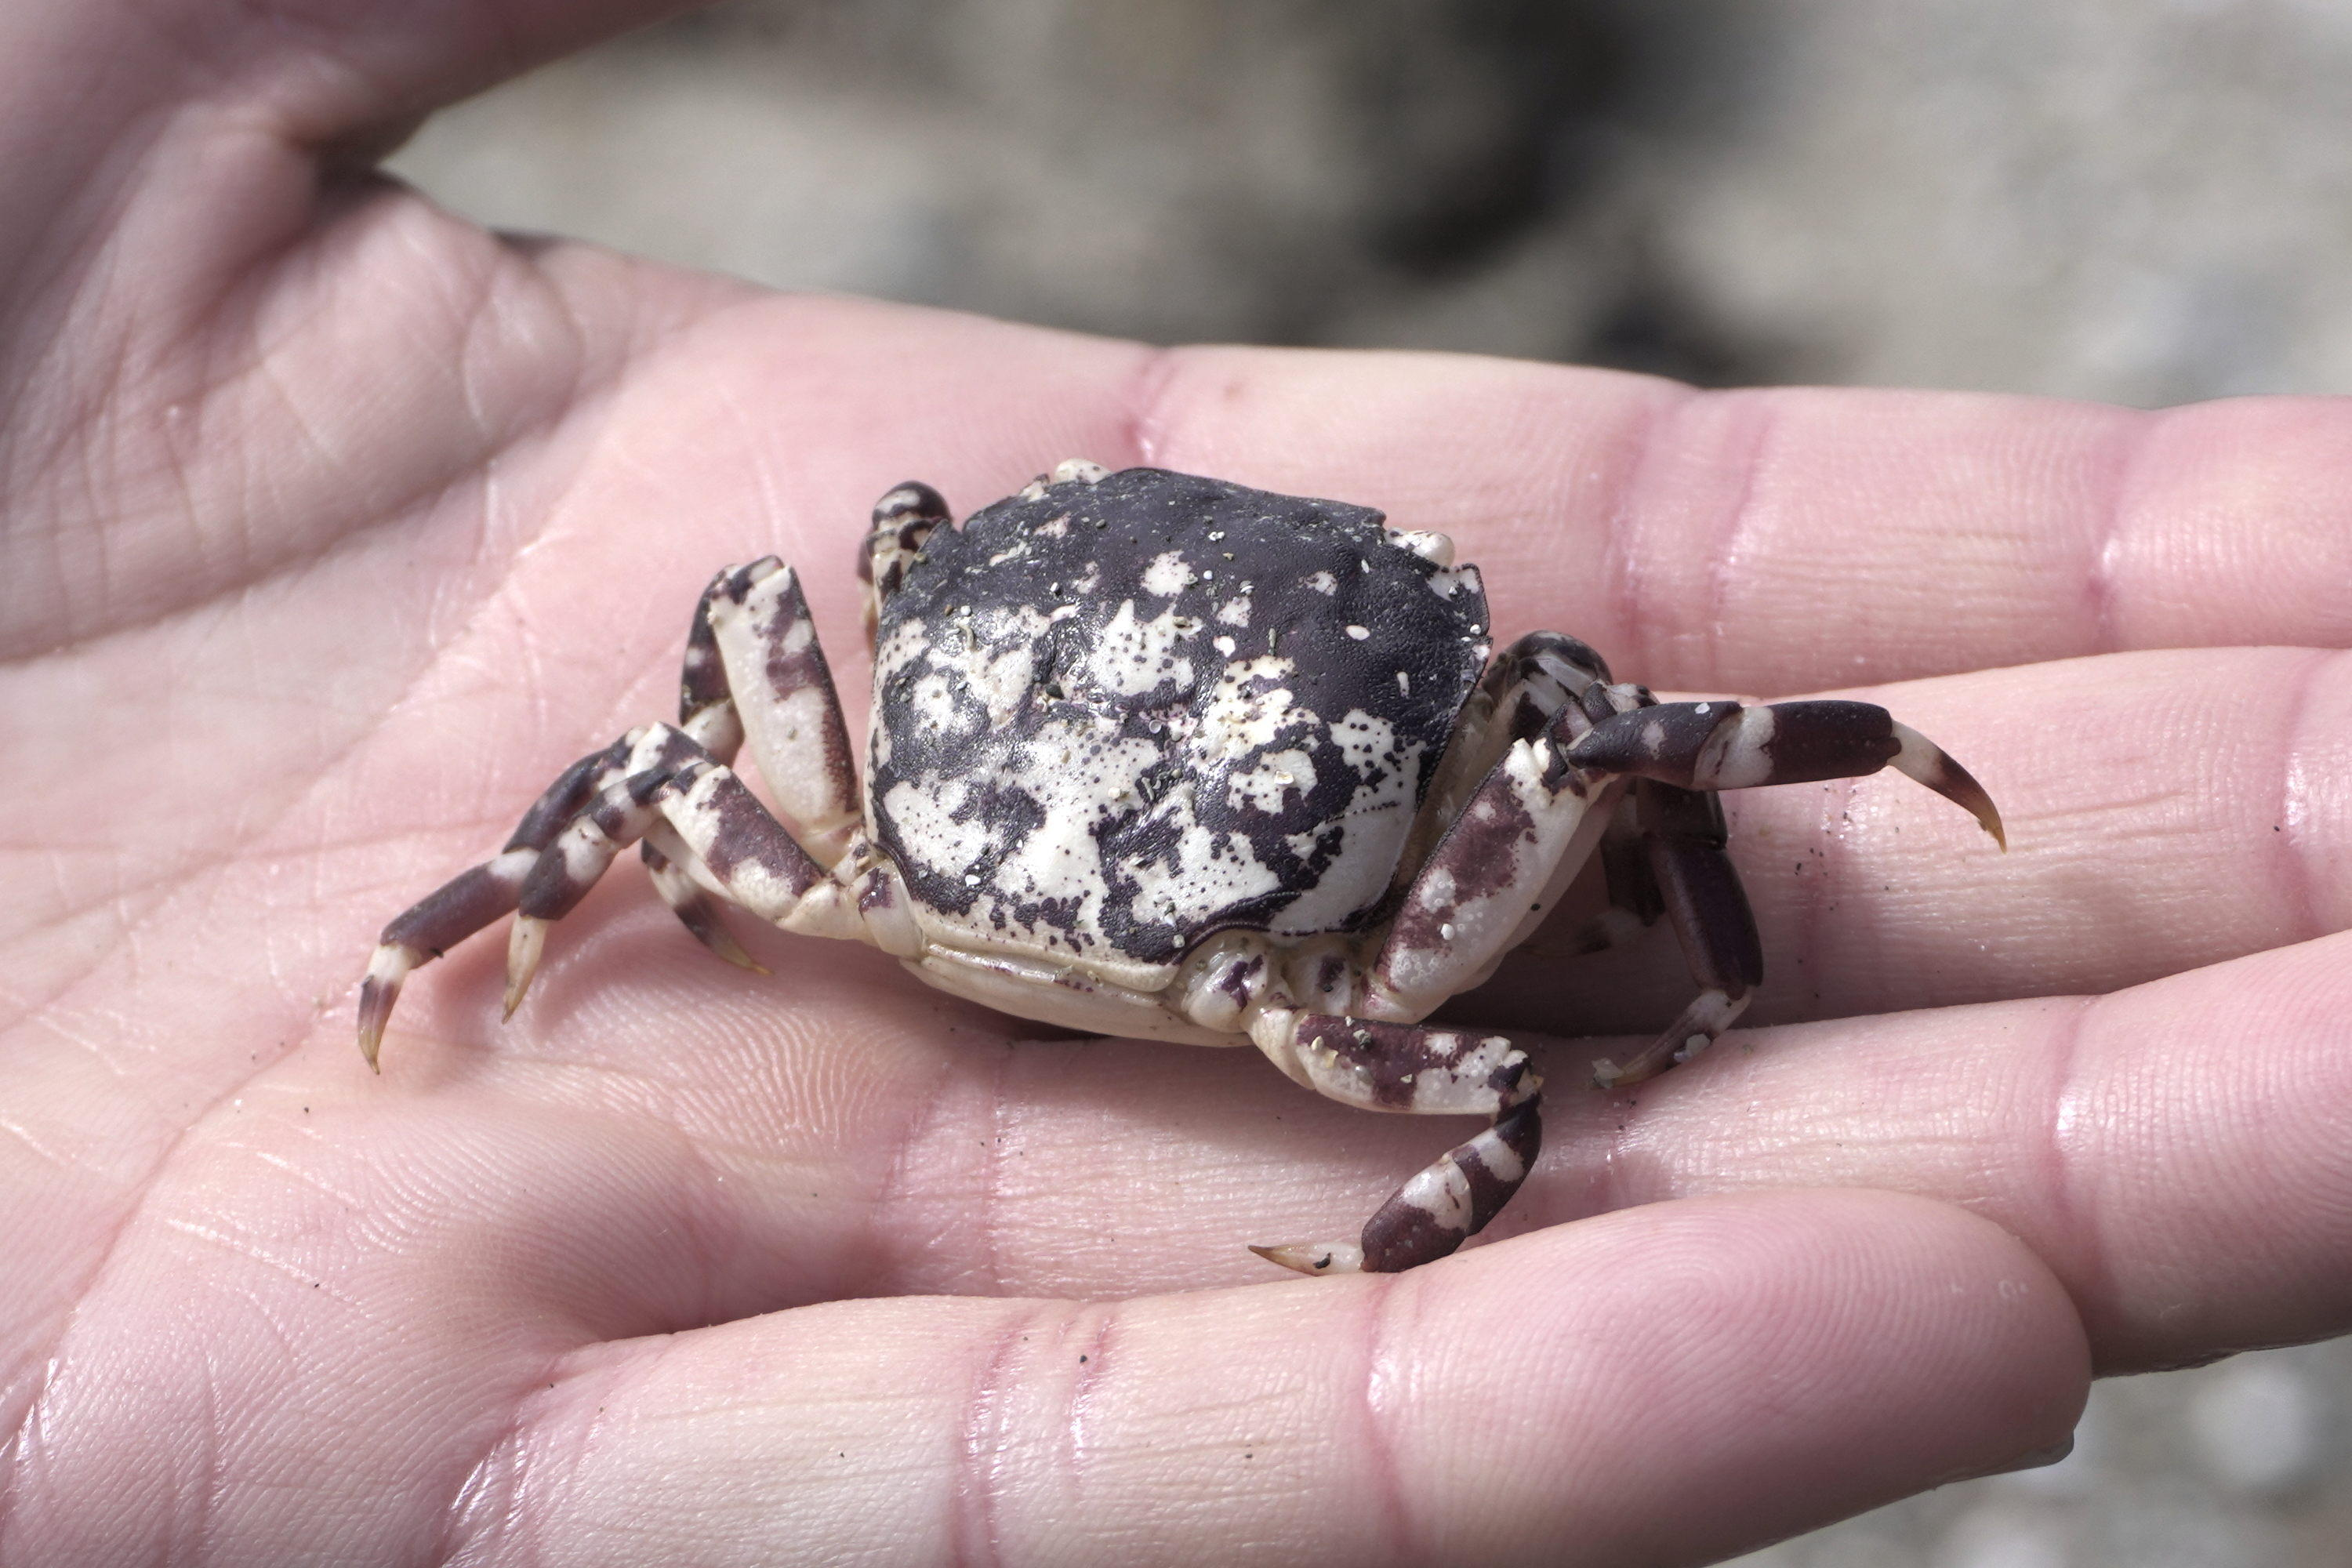
\includegraphics[width=\paperwidth]{L15/02910_smol_common_rock_crab_v1.jpg}};}
\part{Property testing with Bolero;\\ extension to Kani}
\begin{frame}
  \partpage
\end{frame}
%\usebackgroundtemplate{}

\begin{frame}[fragile]
  \frametitle{Last time: Proptest vs proof harness}
  \begin{changemargin}{2cm}
{    \Large
    Let's compare.}
  \end{changemargin}

  \begin{tabular}{ll}
    \scriptsize
      \begin{minipage}{.4\textwidth}
\begin{lstlisting}[language=Rust]
#[cfg(kani)]
#[kani::proof]
fn check_estimate_size() {
    let x: u32 = kani::any();
    estimate_size(x);
}
\end{lstlisting}
      \end{minipage} &
      \begin{minipage}{.4\textwidth}
    \scriptsize
\begin{lstlisting}[language=Rust]
  #[test]
  fn doesnt_crash(x: u32) {
      estimate_size(x);
  }
\end{lstlisting}
      \end{minipage}
    \end{tabular}

  \begin{changemargin}{2cm}
{    \Large
    \ldots still pretty similar! }
  \end{changemargin}

\end{frame}

\begin{frame}
  \frametitle{Bolero}
  \begin{changemargin}{2cm}
    \Large
    meta-framework for property-testing:\\
    integrates fuzzing engines \& also Kani.
  \end{changemargin}
\end{frame}

\begin{frame}[fragile]
  \frametitle{Example: Property testing with Bolero}
{\scriptsize
  Source: \url{https://model-checking.github.io/kani-verifier-blog/2022/10/27/using-kani-with-the-bolero-property-testing-framework.html}.
}

\begin{lstlisting}[language=Rust]
fn update_account_balance(current_balance: i32,
                         amount: i32) -> i32 {
    return current_balance + amount;
}
\end{lstlisting}
\begin{changemargin}{1cm}
  \Large
(Blog post code is not executable, ours sort of is.)
\end{changemargin}
\end{frame}

\begin{frame}[fragile]
  \frametitle{Concrete test}
\begin{lstlisting}[language=Rust]
fn balance_upd_is_correct(current_balance: i32,
   amount: i32, new_balance: i32) -> bool {
 // also: checks other properties
 return current_balance + amount == new_balance; }

#[test]
fn test_update_account_balance() {
 let current_balance = 5; let amount = 2;
 let nb = update_account_balance(current_balance, 
                                 amount);
 assert!(balance_upd_is_correct(current_balance,
                               amount, nb));
}
\end{lstlisting}
\begin{changemargin}{1cm}
  \Large
We can \texttt{cargo test} this, and it succeeds.
\end{changemargin}
\end{frame}

\begin{frame}[fragile]
  \frametitle{DIY random testing}
\begin{lstlisting}[language=Rust]
#[test]
fn test_update_account_balance_random() {
 let current_balance = rand::random();
 let amount = rand::random();
 let result = update_account_balance
                 (current_balance, amount);
 assert!(balance_update_is_correct
                 (current_balance, amount, result));
}
\end{lstlisting}
\begin{changemargin}{1cm}
  \Large
But we've seen better: coverage-guided fuzzing.
\end{changemargin}

\end{frame}

\begin{frame}[fragile]
  \frametitle{Fundamental Theorem of Software Engineering}
  \Large
  \begin{quote}
    ``We can solve any problem by introducing an extra level of indirection.''
  \end{quote}
  \begin{changemargin}{2cm}
    (per Wikipedia, attributed to David J. Wheeler)\\[1em]

    Here: Bolero abstracts away from specific fuzzing engine.
  \end{changemargin}
\end{frame}

\begin{frame}[fragile]
  \frametitle{Bolero at work}
\begin{lstlisting}[language=Rust]
#[test]
#[cfg_attr(kani, kani::proof)]
fn test_update_account_balance_bolero() {
    bolero::check!().with_type::<(i32, i32)>().cloned().for_each(|(current_balance, amount)| {
        let result = update_account_balance(current_balance, amount);
        assert!(balance_update_is_correct(current_balance, amount, result));
    });
}
\end{lstlisting}
\begin{changemargin}{1cm}
  \Large
  I can definitely run this with libfuzzer and Kani. \\
  For technical reasons, AFL doesn't work on my system.\\
  I don't have honggfuzz installed.
\end{changemargin}

\end{frame}

\begin{frame}[fragile]
  \frametitle{Libfuzzer under Bolero}
{ \scriptsize \begin{verbatim}
$ cargo bolero test test_update_account_balance_bolero --engine libfuzzer
\end{verbatim} }

\hspace*{2cm} tells us that our code fails on overflow:

\scriptsize
\begin{verbatim}
======================== Test Failure ========================

Input: 
(
    369098752,
    1778384896,
)

Error: 
panicked at src/main.rs:6:12:
attempt to add with overflow
note: run with `RUST_BACKTRACE=1` environment variable to display a backtrace.
\end{verbatim}
\end{frame}

\begin{frame}[fragile]
  \frametitle{Kani under Bolero}
  \scriptsize
\begin{verbatim}
$ cargo bolero test test_update_account_balance_bolero --engine kani
[...]
SUMMARY:
 ** 1 of 238 failed (1 unreachable)

 ** 1 of 1 cover properties satisfied

Failed Checks: attempt to add with overflow
 File: "src/main.rs", line 6, in update_account_balance

VERIFICATION:- FAILED
Verification Time: 0.16379055s
\end{verbatim}
\end{frame}

\begin{frame}[fragile]
  \frametitle{Another Bolero example: nth-rev}
  \begin{changemargin}{1cm}
    (Incorrectly) return $n$\textsuperscript{th}-from-the-end element as \texttt{Some(x)}.
  \end{changemargin}
\small \begin{lstlisting}
fn nth_rev(arr: &[i32], index: usize) -> Option<i32> {
    if index < arr.len() {
        let rev_index = arr.len() - index /* - 1 */;
        return Some(arr[rev_index]);
    }
    None
}
\end{lstlisting}
\end{frame}

\begin{frame}[fragile]
  \frametitle{Bolero harness}
  \begin{changemargin}{1cm}
{\Large    Check that we get \texttt{Some()} from each element.}
  \end{changemargin}
  \small
\begin{lstlisting}
const N: usize = 5; // bound for BMC

#[test]
#[cfg_attr(kani, kani::proof)] // if Kani, mark as proof harness
fn check_rev() {
    bolero::check!()
        .with_type::<([i32; N], usize)>()
        .cloned()
        .for_each(|(arr, index)| {
            let x = nth_rev(&arr, index);
            if index < arr.len() {
                assert!(x.is_some());
            }
        });
}
\end{lstlisting}
\end{frame}

\begin{frame}[fragile]
  \frametitle{libfuzzer finds the bug}
  \begin{changemargin}{1cm}
\scriptsize \begin{verbatim}
$ cargo bolero test check_rev --engine libfuzzer
[...]
test failed; shrinking input...

======================== Test Failure ========================

Input: 
(
    [
        0,
        0,
        0,
        0,
        0,
    ],
    0,
)

Error: 
panicked at src/main.rs:8:21:
index out of bounds: the len is 5 but the index is 5
\end{verbatim}
  \end{changemargin}
\end{frame}

\begin{frame}[fragile]
  \frametitle{Kani finds the bug}
  \begin{changemargin}{1cm}
\scriptsize 
\begin{verbatim}
$ cargo bolero test check_rev --engine kani
[...]
SUMMARY:
 ** 1 of 698 failed (8 unreachable)

 ** 1 of 1 cover properties satisfied

Failed Checks: index out of bounds: the length is less than or equal to the given index
 File: "src/main.rs", line 8, in nth_rev

VERIFICATION:- FAILED
Verification Time: 1.0711443s
\end{verbatim}
  \end{changemargin}
\end{frame}

\begin{frame}[fragile]
  \frametitle{After fixing, Kani succeeds}
  \begin{changemargin}{1cm}
\scriptsize 
\begin{verbatim}
SUMMARY:
 ** 0 of 699 failed (8 unreachable)

 ** 1 of 1 cover properties satisfied


VERIFICATION:- SUCCESSFUL
Verification Time: 1.0993001s
\end{verbatim}

\Large ~ \\[1em]
libfuzzer also doesn't find any bugs on an overnight run.
  \end{changemargin}
\end{frame}

\begin{frame}[fragile]
  \frametitle{Why both Kani and libfuzzer}
  \begin{changemargin}{1cm}
    \Large
    My take:
    \begin{itemize}
    \item Kani and libfuzzer succeeded and failed on same programs.
      \item This is not true in general.
    \end{itemize}
    Perhaps fuzzing doesn't find anything, \\ but Kani does.\\[1em]
    Or, Kani might not find an issue, \\
    but fuzzing does.
  \end{changemargin}
\end{frame}

\begin{frame}[fragile]
  \frametitle{Outputs from Kani and libfuzzer}
  \begin{changemargin}{1cm}
    \large
    Both fuzzing and Kani might give a test case; \\
    it's real, and you can fix it.\\[1em]
    Unwinding assertion failure: must investigate more.\\
    Kani success: your program is correct modulo the bound,\\
    assuming everything else on the system correct.\\[1em]
    Fuzzing says nothing: don't really know that your program is correct,
    but have some warm and fuzzy feelings.
  \end{changemargin}
\end{frame}

\begin{frame}[fragile]
  \frametitle{Under the hood: Bolero \& Kani}
  \begin{changemargin}{1cm}
    \Large
    Bolero uses \texttt{kani::any()} to get a symbolic value, \\
    \hspace*{1em} \texttt{kani::assume()} to restrict the range, e.g.
    \normalsize
\begin{lstlisting}
  bolero::check!().with_generator(5..37)
      .for_each( // snip... );
\end{lstlisting}
\Large becomes \normalsize
\begin{lstlisting}
  let value = kani::any();
  kani::assume((5..37).contains(&value));
  value
\end{lstlisting}
  \end{changemargin}
\end{frame}
    
\part{Kani (BMC) to Dafny (auto-active program verification)}
\begin{frame}
  \partpage
\end{frame}

\begin{frame}
  \frametitle{About Dafny}

  \Large
  \begin{changemargin}{1cm}
    Dafny: automatically verify annotated programs.\\[1em]
    In SE212, manually (with George's help) prove programs.\\[1em]
    Dafny does the same, but mostly automatically.\\[1em]
    Terminology: ``auto-active'' (versus interactive).
  \end{changemargin}
\end{frame}

\begin{frame}[fragile]
  \frametitle{Kani vs Dafny: Rust Rectangle example}
\small
\begin{lstlisting}[language=Rust]
#[derive(Debug, Copy, Clone)]
struct Rectangle {
    width: u64, height: u64,
}

impl Rectangle {
    fn can_hold(&self, other: &Rectangle) -> bool {
        self.width > other.width && 
        self.height > other.height 
    }

    fn stretch(&self, factor: u64) -> Option<Self> {
        let w = self.width.checked_mul(factor)?;
        let h = self.height.checked_mul(factor)?;
        Some(Rectangle {
            width: w,
            height: h,
        })
    }
}
\end{lstlisting}
\end{frame}
\begin{frame}[fragile]
  \frametitle{Dafny Rectangle}
\large
\begin{lstlisting}[language=dafny]
  class Rectangle {
      var width:int
      var height:int
  }

  predicate can_hold(self:Rectangle, other:Rectangle)
      reads self, other
  {
      self.width > other.width && self.height > other.height
  }

  method stretch(self:Rectangle, factor:nat)
           returns (rv : Rectangle) {
      rv := new Rectangle;
      rv.width := self.width * factor;
      rv.height := self.height * factor;
      return rv;
  }
\end{lstlisting}
\end{frame}

\begin{frame}[fragile]
  \frametitle{Rust concrete test case}
  \begin{changemargin}{1cm}
    Just an average test case.
  \end{changemargin}
  \small
\begin{lstlisting}[language=Rust]
  #[cfg(test)]
  mod tests {
      use super::*;

      #[test]
      fn stretched_rectangle_can_hold_original() {
          let original = Rectangle {
              width: 8,
              height: 7,
          };
          let factor = 2;
          let larger = original.stretch(factor);
          assert!(larger.unwrap().can_hold(&original));
      }
  }
\end{lstlisting}
\end{frame}

\begin{frame}[fragile]
  \frametitle{Dafny concrete test case}
  \begin{changemargin}{1cm}
    Just an average test case (in Dafny).
  \end{changemargin}
  \small
\begin{lstlisting}[language=dafny]
method {:test} TestStretchedRectangleCanHoldOriginal() {
    var original := new Rectangle;
    original.width := 8; original.height := 7;
    var factor := 2;
    var larger := stretch(original, factor);
    expect can_hold(larger, original);
}
\end{lstlisting}
\large
  \begin{changemargin}{1cm}
    Note: \texttt{expect} is dynamic \texttt{assert}; plain \texttt{assert} is static.\\[1em]
    More generally: the concrete test case is concrete; \\
    we can write \texttt{assert}, in which case
    we need the method to have an \texttt{ensures} clause.\\[1em]
    If we have \texttt{ensures} then we can verify the whole method under all inputs.
  \end{changemargin}
\end{frame}

\begin{frame}[fragile]
  \frametitle{Back to proptests: this works}
\begin{lstlisting}[language=Rust]
#[cfg(test)]
mod proptests {
 use super::*;
 use proptest::prelude::*;
 use proptest::num::u64;

 proptest! {
   #[test]
   fn stretched_rectangle_can_hold_original
      (width in u64::ANY, height in u64::ANY,
       factor in u64::ANY) {
     let original = Rectangle {
       width: width, height: height,
     };
     if let Some(larger) = original.stretch(factor) {
       assert!(larger.can_hold(&original));
     } } } }
\end{lstlisting}
\end{frame}

\begin{frame}[fragile]
  \frametitle{All the way to Kani}
\begin{lstlisting}[language=Rust]
// cargo kani --harness stretched_rectangle_can_hold_original}.
#[cfg(kani)]
mod verification {
 use super::*;

 #[kani::proof]
 pub fn stretched_rectangle_can_hold_original() {
  let original = Rectangle {
      width: kani::any(),
      height: kani::any(),
  };
  let factor = kani::any();
  if let Some(larger) = original.stretch(factor) {
      assert!(larger.can_hold(&original));
  } } }
\end{lstlisting}
\end{frame}

\begin{frame}[fragile]
  \frametitle{Proof harness implications}
  \begin{changemargin}{1cm}
    \Large
    Kani verifies behaviour for \emph{any} width, height, and factor.\\[1em]
    It runs a whole bunch of tests, looking for safety violations (because Unsafe Rust).\\[1em]
    But, also reports a failure!
{ \scriptsize
\begin{verbatim}

Check 3: verification::stretched_rectangle_can_hold_original.assertion.1
	 - Status: FAILURE
	 - Description: "assertion failed: larger.can_hold(&original)"
	 - Location: src/lib.rs:72:13 in function verification::stretched_rectangle_can_hold_original
[...]
SUMMARY:
 ** 1 of 40 failed
Failed Checks: assertion failed: larger.can_hold(&original)
 File: "src/lib.rs", line 72, in verification::stretched_rectangle_can_hold_original

VERIFICATION:- FAILED
Verification Time: 0.08609796s
\end{verbatim}
}
  \end{changemargin}
\end{frame}

\begin{frame}[fragile]
  \frametitle{Why failure?}
  \begin{changemargin}{1cm}
    \Large
    We're missing some preconditions.\\[1em]
    We'll encode them directly into the harnesss:
\begin{lstlisting}[language=Rust]
kani::assume(0 != original.width);
kani::assume(0 != original.height);
kani::assume(1 < factor);          
\end{lstlisting}

With these \textsf{assume}s (effectively preconditions), Kani verifies the code.
  \end{changemargin}
\end{frame}

\begin{frame}[fragile]
  \frametitle{Analogous Dafny}
  \small
\begin{lstlisting}[language=dafny]
method stretch(self:Rectangle, factor:nat) returns (rv : Rectangle)
    ensures rv.width == self.width * factor && 
            rv.height == self.height * factor
{
    rv := new Rectangle;
    rv.width := self.width * factor;
    rv.height := self.height * factor;
    return rv;
}

method stretched_rectangle_can_hold_original
                (original:Rectangle, factor:nat)
    requires original.width > 0 && 
             original.height > 0 && factor > 1
{
    var larger := stretch(original, factor);
    assert can_hold(larger, original);
}
\end{lstlisting}
\end{frame}

\usebackgroundtemplate{\tikz\node[opacity=0.3]{
\includegraphics[width=\paperwidth]{L17/PXL_20220729_181423529.jpg}};}
\part{Dafny application: Cedar authorization-policy}
\begin{frame}
  \partpage
\end{frame}
\usebackgroundtemplate{}

\begin{frame}[fragile]
  \frametitle{Cedar: a use of Dafny in practice}
    \Large
  \begin{changemargin}{1cm}
    At Amazon: Cedar authorization-policy language in Dafny.\\[1em]
    Later: migrated to Lean, interactive theorem proving---more powerful.\\[1em]
  \end{changemargin}
    {\scriptsize \url{https://www.amazon.science/blog/how-we-built-cedar-with-automated-reasoning-and-differential-testing}\\[1em]}

  \begin{changemargin}{1cm}
    Cedar: write policies in domain-specific language;\\
    execute queries on these policies;\\
    response: ``allow'' or ``deny''.
  \end{changemargin}
\end{frame}

\begin{frame}[fragile]
  \frametitle{Cedar policy: TinyTodo policy 1 (allow)}
\large
\begin{verbatim}
// policy 1: enables access sometimes
permit(principal, action, resource)
when {
  resource has owner &&
  resource.owner == principal
};
\end{verbatim}
\begin{changemargin}{1cm}
  principal is a User\\
  resource is a List\\
\end{changemargin}
\end{frame}

\begin{frame}[fragile]
  \frametitle{Cedar policy: TinyTodo policy 3 (deny)}
    \large
\begin{verbatim}
// policy 3
forbid (
  principal in Team::"interns",
  action == Action::"CreateList",
  resource == Application::"TinyTodo"
);
\end{verbatim}
\end{frame}

\begin{frame}[fragile]
  \frametitle{TinyTodo and Cedar}
    \Large
    \begin{changemargin}{2cm}
      Idea: given policies in the DSL,\\
      TinyTodo doesn't contain reasoning about auth.\\[1em]
      Just ask Cedar about whether an action is allowed or denied (and listen to it.)
    \end{changemargin}
\end{frame}

\begin{frame}[fragile]
  \frametitle{Verification-guided development}
    \Large
    \begin{changemargin}{2cm}
      Dafny (and Lean): prove properties of software.\\[1em]
      Specifically: there are
      \begin{enumerate}
      \item explicit properties (specified by developers); and
      \item implicit properties (must always be true).
      \end{enumerate}

      Get formal guarantees---better than testing, if you can prove them.
    \end{changemargin}
\end{frame}

\begin{frame}[fragile]
  \frametitle{Deployment and models}
    \Large
    \begin{changemargin}{2cm}
      Usually don't want to deploy raw Dafny.\\[1em]
      Fortunately, Dafny compiles to C\#, Java, JavaScript, Go, and Python.\\[1em]
      In the Cedar example: Dafny is a model of the Rust code.\\[1em]
      Verifying the Dafny is still useful; it implies that a correct implementation is possible.
    \end{changemargin}
\end{frame}

\begin{frame}[fragile]
  \frametitle{Using the Dafny}
    \Large
    \begin{changemargin}{2cm}
      Dafny code, especially verified, can serve as an oracle.\\
      We can look for divergences between Dafny \& Rust.\\[1em]

      Really, we want to know that the Rust code satisfies the properties.\\[1em]
      Safe Rust: no undefined behaviour.\\
      But what about contracts?
    \end{changemargin}
\end{frame}

\begin{frame}[fragile]
  \frametitle{Assertions in Rust}
    \Large
    \begin{changemargin}{2cm}
      Sure, but what if they fail?
    \end{changemargin}
\end{frame}


\begin{frame}[fragile]
  \frametitle{Idea: \alert{differential random testing}}
    \Large
    \begin{changemargin}{2cm}
      Make sure that the Rust implementation matches the Dafny model.\\[1em]
      Like fuzzing: generate millions of inputs, check equivalence.
    \end{changemargin}
\end{frame}

\begin{frame}[fragile]
  \frametitle{Key properties of Cedar}
    \Large
    \begin{changemargin}{2cm}
      Two overarching properties:
      \begin{itemize}
      \item \alert{explicit permit}: permission granted only by individual \emph{permit} policies, not gained by error or default;
      \item \alert{forbid overrides permit}: any applicable \emph{forbid} policy always denies access, even if \emph{permit} policy allows it.
      \end{itemize}
      That is: authorization has to be explicitly granted by a specific policy; but if there is any forbid policy, then access is forbidden.
    \end{changemargin}
\end{frame}

\begin{frame}[fragile]
  \frametitle{Example Request}
    \Large
    \begin{changemargin}{2cm}
      \textit{principal=}\textbf{User::``Alice"}\\
      \textit{action=}\textbf{Action::``GetList"}\\
      \textit{resource=}\textbf{List::``AliceList"}\\[1em]

      Policy 1 yields \textbf{List::``AliceList" has owner \&\& List::``AliceList".owner == User::``Alice"}\\[1em]
      
      Say this is true. The request then \emph{satisfies} the policy. \\[1em]

      More generally, the authorization engine computes the request over all of its policies and returns an overall decision.
    \end{changemargin}
\end{frame}

\begin{frame}[fragile]
  \frametitle{Buggy Dafny Code}
    \Large
\begin{lstlisting}[language=dafny]
function method isAuthorized(): Response { // BUGGY VERSION
  var f := forbids();
  var p := permits();
  if f != {} then
    Response(Deny, f)
  else
    Response(Allow, p)
}
\end{lstlisting}
\begin{changemargin}{2cm}
  Why is this wrong with respect to earlier properties?
\end{changemargin}
\end{frame}

\begin{frame}[fragile]
  \frametitle{Patching with a predicate}
    \Large
\begin{lstlisting}[language=dafny]
// A request is explicitly permitted when a permit policy is satisfied
predicate IsExplicitlyPermitted(request: Request, store: Store) {
  exists p ::
    p in store.policies.policies.Keys &&
    store.policies.policies[p].effect == Permit &&
    Authorizer(request, store).satisfied(p)
}

lemma AllowedIfExplicitlyPermitted(request: Request, store: Store)
ensures // A request is allowed if it is explicitly permitted
	(Authorizer(request, store).isAuthorized().decision == Allow) ==>
	IsExplicitlyPermitted(request, store)
{ ... }
\end{lstlisting}
\end{frame}

\begin{frame}[fragile]
  \frametitle{Trying to verify isAuthorized}
  \large
  \begin{changemargin}{1cm}
    Predicate \texttt{isExplicitlyPermitted}: there has to be a specific policy \texttt{p} which permits \texttt{request}.\\[1em]
    
Lemma \texttt{AllowedIfExplicitlyPermitted} needs to be shown---i.e. if authorizer says yes,
then predicate \texttt{IsExplicitlyPermitted} has to be true. \\[1em]

When Dafny verifies  \texttt{isAuthorized}, it tries to check that the lemma.\\[1em]

But the lemma doesn't hold, so Dafny will report ``A postcondition might not hold on this return path'', pointing at the
ensures clause.
  \end{changemargin}
\end{frame}

\begin{frame}[fragile]
  \frametitle{Fixing isAuthorized}
\begin{center}
\begin{minipage}{.45\textwidth}
\begin{lstlisting}[language=dafny]
  // BUGGY VERSION
  function method isAuthorized():
       Response { 
  var f := forbids();
  var p := permits();
  if f != {} then
    Response(Deny, f)
  else
    Response(Allow, p)
}
\end{lstlisting} \end{minipage} \begin{minipage}{.45\textwidth}
  \begin{lstlisting}[language=dafny]
  // FIXED VERSION
  function method isAuthorized():
       Response {
    var f := forbids();
    var p := permits();
    if f == {} && p != {} then
      Response(Allow, p)
    else
      Response(Deny, f)
}
  \end{lstlisting}
\end{minipage}
\end{center}
Dafny verifies the fixed version, and also the mirror property \emph{forbid overrides permit}, which we don't show.
\end{frame}

\begin{frame}[fragile]
  \frametitle{What Dafny shows}
  \Large
  \begin{changemargin}{2cm}
    Other properties, notably that the Cedar validator is sound:\\[1em]
    ``if the validator accepts a policy, evaluating the policy should never result in certain classes of error.''\\[1em]

    Making this proof go through enabled developers to fix subtle design bugs, which would otherwise be reflected in the implementation.
  \end{changemargin}
\end{frame}

\begin{frame}[fragile]
  \frametitle{Usefulness of Dafny}
  \Large
  \begin{changemargin}{2cm}
    We can use the specification for:
    \begin{itemize}
      \item automated reasoning, by Dafny; but also
      \item manual reasoning, by people.
    \end{itemize}

    Even good Rust is still an implementation language with lots of implementation details.

Reading the Dafny (or Lean) is much easier, since it has much less code (1/6th, at time of report).
  \end{changemargin}
\end{frame}

\begin{frame}[fragile]
  \frametitle{Dafny and Rust}
  \large
  \begin{changemargin}{1cm}
    Are they the same?\\[1em]
    If you don't know, bugs can sneak into the implementation.\\[1em]
    Solution: \alert{differential random testing} (DRT).\\[1em]

    That is: randomly generate millions of inputs (access requests, data, and policies);\\
    check that Dafny (now Lean) and Rust produce the same output.\\
    If they disagree, that's a bug.\\[1em]
  \end{changemargin}
\end{frame}

\begin{frame}[fragile]
  \frametitle{More on differential random testing}
  \large
  \begin{changemargin}{1cm}
      Inputs aren't completely randomly generated. \\
      Same techniques as talked about in this class: input generators to create consistent inputs.\\
      6 hours nightly of DRT, 100 million total tests.\\[1em]
      Found errors in libraries (mostly parsers and IP address operations).
  \end{changemargin}
\end{frame}

\begin{frame}[fragile]
  \frametitle{Cedar Summary}
  \Large
  \begin{changemargin}{1cm}
    Cedar policy-authorization language.\\[1em]
    Modelled in Dafny, showing key properties.\\[1em]
    Rust implementation shown equivalent to Dafny using differential random testing.
  \end{changemargin}
\end{frame}
\end{document}
